\section{Research Method} \label{sec:research_method}

We adopted Grounded Theory (GT) as the research method. GT is a method originally
proposed by Glase~\cite{glase1967discovery}, which has as distinguishing features (1) the
absence of clear research hypothesis upfront and (2) limitation of literature
exposure at the beginning of the research. GT is a theory-developing approach in
contrast with the more traditional theory-testing approach
\cite{coleman2007using}.\gnote{não sei se entendi a diferenca. algum exemplo?}
We used GT as the research method due to the following reasons:

%Some of related work claimed to used ``GT inspired'' approaches\gnote{REF}. It is a very
%common rhetoric in recent research on software engineering, but only research
%that embodies GT’s core principles should claim to be a grounded theory study
%\cite{stol2016grounded}.\gnote{eu removi esse paragrafo pq acho que ele facilmente compraria briga com muitos revisores}


\begin{itemize}

\item GT is a consolidated method in other areas of research like sociology\gnote{REF},
nursing\gnote{REF}, education\gnote{REF}, and finances\gnote{REF}. GT is also increasingly being employed
to study software engineering topics~\cite{Hoda:2017:ICSE,stol2016grounded,Waterman:2015:ICSE};

\item GT is considered an adequate approach to investigate scenarios with
questions such as ``\textit{what's going on here?}''~\cite{barnsteiner2002using},
which is exactly the scenario proposed here: what's going on DevOps adoption?

\item GT allows researchers to get descriptions\gnote{what is this get descriptions?} without bias of previous
researches, which is adequate to collect empirical evidence directly from the
practice on industry\gnote{nao entendi bem a relação do primeiro item com o segundo?}. The evidence is only reintegrated back with literature
after the theory construction.

\end{itemize}

Since the publication of the Glase's original version~\cite{glase1967discovery},
several modifications and variations occurred in the original text, coming to
exist at least seven different versions of the GT method~\cite{denzin2007grounded}.
The main versions are those of Glaser, Strauss and
Charmaz~\cite{stol2016grounded}. The study of Stol and colleagues~\cite{stol2016grounded}
explores the main aspects of GT versions and establishes that GT studies has to
specify which version the study is built upon. In our study, we chose the classic
Glase's version due to at least two reasons.


\begin{enumerate}
\item First because we did not have a research
question at the beginning of the research, exactly as suggested in the classic
version. We start from an area of interest: successfully DevOps adoption
in industry.
\item Second because the more detailed papers in
software engineering research use predominantly this version~\cite{stol2016grounded}.
\end{enumerate}


\subsection{GT Procedures}

In Figure~\ref{fig1}, reproduced from the study of Adolph and colleagues~\cite{adolph2011using}, shows the procedure of the grounded theory research methods followed in the conduction of this
research.

\begin{figure}[htpb]
  \centering
  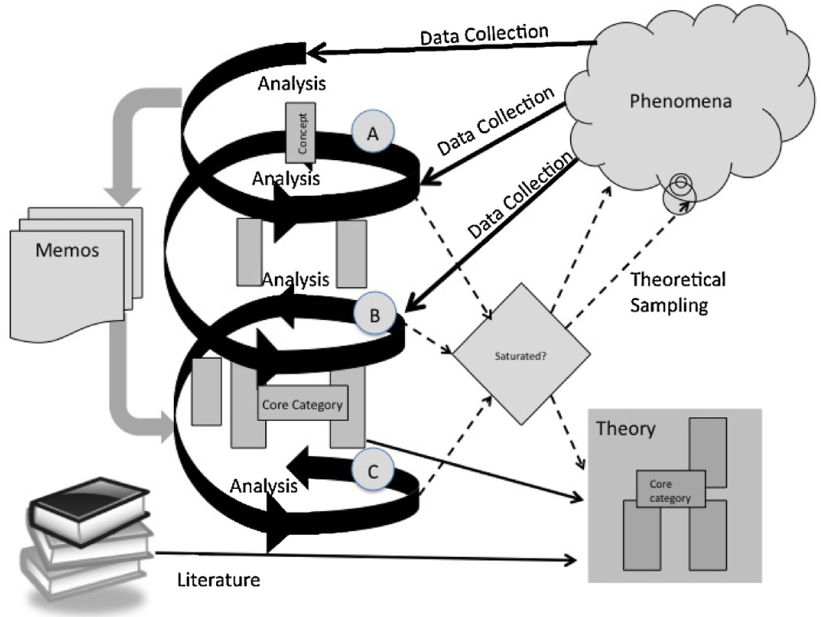
\includegraphics[width=0.5\textwidth,natwidth=821,natheight=617]{GT.png}
  \caption{The GT Method (reproduced from the study of Adolph and colleagues~\cite{adolph2011using}).}
  \label{fig1}
\end{figure}

This figure depicts four main steps (enumerated as A -- D).

\gnote{acho que antes disso, é preciso dizer como você encontrou e abordou
os possiveis entrevistados? Jogou um convite nas redes socias? foi por
conveniencia (p.e., vc conhecia alguem?), etc}

\begin{enumerate}[label=(\Alph*)]
\item Initially, we begin collecting data about the adoption process from
companies that have successfully adopted it. As the data were collected, they
were also analyzed simultaneously. The raw data is analyzed by searching for
patterns of incidents to indicate concepts, and concepts grouped into
categories. This first step, where all raw data is analyzed, is called open
coding~\cite{stol2016grounded}.

\item The categories are developed by constant comparison of new incidents with
previous. Every grounded theory study has to identify a ``core category"~\cite{stol2016grounded}.
The core category is responsible for enabling the
integration of the other categories and structuring the results into a dense
and consolidated grounded theory~\cite{jantunen2014using}. The identification
of the core category represents the end of open coding and the beginning of the
selective coding. In selective coding, only specific variables that are
directly related to the core category and their relationships are coded, in
order to enable the production of a harmonic theory~\cite{coleman2007using,hoda2011impact}.
Selective coding ends when theoretical saturation is achieved, which occurs when new data (............). Theoretical coding....

\item After saturation, the resulting theory is reintegrated back into
literature comparing with existing theories. The literature search is performed
only later to avoid forcing preconceived concepts on the theory development~\cite{adolph2012reconciling}.

\item Throughout the process, memos were wrote capturing thoughts and analytic
processes; the memos support the emerging concepts, categories, and their
relationships~\cite{adolph2012reconciling}.
\end{enumerate}

\gnote{para cada um dos itens acima, poderiamos colocar exemplos reais
do trabalho? p.e., citar 1-2 memos?}

The following sub-sections present details of procedures applied in this study,
containing some examples to illustrate their application.

\subsection{Data Collection}
We conducted semi-structured interviews with 15 practitioners of companies from
Brazil, Portugal, Ireland, United States, and Spain. This practitioners claim
to have participated to DevOps adoption process in their companies. Participants
were recruited using two approaches: (1) through direct contact in DevOps days event
and (2) through  general
calls for participation posted on DevOps user groups, social networking sites
and local communities. A variety of company types were covered in order to
achieve a heterogeneous perspective, increasing the potential of generalization
of the results. Table~\ref{participant_table} presents the participant
characteristics.


\begin{table}[t]
\centering
\caption{Participant Profile. SWX means software development experience in years, DX means DevOps experience in years, CN means country of work, and CS means company size (CS).}
\label{participant_table}
\begin{tabular}{ccccccc}
\textbf{P\#}          & \textbf{Role}         & \textbf{SWX} & \textbf{DX} & \textbf{CN}   & \textbf{Domain}    & \multicolumn{1}{l}{\textbf{CS}} \\
P1                   & DevOps Developer      & 9            & 2           & IR            & IT                 & S                               \\

P2                   & DevOps Consultant       & 9            & 3           & BR            & IT                 & M                               \\

P3                   & DevOps Developer      & 8            & 1           & IR            & IT                 & S                               \\

P4                   & Computer Tech.        & 10           & 2           & BR            & Health             & S                               \\

P5                   & Systems Engineer      & 10           & 3           & SP            & Telecom            & XL                              \\

P6                   & Developer             & 3            & 1           & PO            & IT                 & S                               \\

P7                   & Support Analyst       & 15           & 2           & BR            & Telecom            & L                               \\

P8                   & DevOps Engineer       & 20           & 9           & BR            & Imob?              & M                               \\

P9                   & IT Manager            & 14           & 8           & BR            & IT                 & M                               \\

P10                  & Network Admin.        & 15           & 3           & BR            & IT                 & S                               \\

P11                  & DevOps Supervisor                & 6            & 4           & BR            & IT                  & M                               \\

P12                  & Cloud Engineer              & 9            & 3           & US            & IT                  & L                               \\

P13                  & Technology Manager                 & 18            & 6           & BR            & Food                  & M                               \\

P14                  & IT Manager            & 7            & 2           & BR            & IT                  & S                               \\

P15                  & Developer        & 3            & 2           & BR            & IT                  & S
\end{tabular}
\end{table}


To maintain anonymity in conformance with the human ethics guidelines,
we refer to the participant as P1--P15 (first column).
The second column shows the role of
each participant in her respective company. The remaining columns list their
software development experience in years (SWX), DevOps experience in years (DX),
country of work (CN), main domain of the company \gnote{o que seria o asterístico na tabela?}, and company
sizes (CS).


The interview were conducted over one year using Skype calls and lasted
approximately 30 minutes on average (max? min?).

Data collection and analysis were iterative so the collected data helped guide
future interviews. The questions of interview evolved according to the progress
of the research...

\subsection{Data Analysis}
The interviews were voice recorded, transcribed, and analyzed. The first moment
of the analyze, called open coding in GT, started immediately after

transcription of the first interview. The analysis of the
first interview was used to evolve the interview script to be used in
the second interview, and so on.

The open coding lasted until there was no doubt about the core category of the
study. Similar to what is described in the work of adolph and colleagues\cite{adolph2012reconciling}, we  started with a strong candidate core category yet not consolidated. Until
the analysis of the fourth interview, we cogitated automation as core
category because it is a recurring pattern in our data. However, we quickly
realized that the ``automation" category did not explain most of the behaviors
or events in our data. At the same time we start to perceive that the
collaboration culture also appeared recurrently in the analysis and with more
potential to explain the remaining events. We then started to ask explicitly
about the role of the automation and how the collaboration culture is formed
in a DevOps adoption process.

After the adaptations made in the script and analysis of new data in a constant
comparison process, taking into account the previous analyses and the

respective memos wrote during all the process, during the analysis of the tenth
interview, we concluded that ``collaboration culture" was unequivocal the core
category regarding how DevOps was
successfully adopted in the studied companies. At this moment, the open coded ended and the selective coding started.

After the discovery of the core category, we started to restrict the coding only
to specific variables that are directly related to the core category and their
relationships: the selective coding.

With more three interviews and respective analysis, we realized that
the new data added less and less content to the emerging theory. The
explanation around how the collaboration culture is developed providing
DevOps adoption showed signs of saturation. We then conducted more two
interviews to conclude that we had reached the theoretical saturation.

After saturation, we started the theoretical coding to find a way to integrate
all the concepts, categories and memos in the form of a cohesive and
homogeneous theory, where we have pointed out the role of the categories as
enablers and outcomes, as shown above.

To illustrate the coding procedures, we present an example of working from
interview transcript to the findings for one of the categories: automation.

\gnote{seria bom linkar aqui os itens A--B descritos na seção anterior.}

Apresentar aqui a exemplificacao da codificacao....

\subsection{Reintegrate with Literature (?)}
